%----------------------------------------------------------
% Research Proposal: Multi-Path Ring-Based Algorithms for Data-Center Networks
%----------------------------------------------------------
\documentclass[12pt]{article}

%----------- Packages and Layout -------------------------
\usepackage[utf8]{inputenc}
\usepackage[T1]{fontenc}
\usepackage{geometry}
\usepackage{amsmath,amssymb,amsthm}
% For algorithms: enable ruled style, vertical lines and line numbers for better readability
\usepackage[ruled,vlined]{algorithm2e}
\SetAlgoLined
\DontPrintSemicolon
\usepackage{parskip}       % Better paragraph spacing
\usepackage{booktabs}      % Professional tables
\usepackage{array}         % Improved array handling
\usepackage{enumitem}      % Customizable lists
\usepackage{ragged2e}      % Improved text alignment
\usepackage{graphicx}      % For figures
\usepackage{subcaption} % for side-by-side subfigures
\usepackage{xcolor}
\usepackage{fancyhdr}      % Headers and footers

\usepackage[backend=biber,style=ieee,sorting=none,maxnames=8,giveninits=true]{biblatex}
\addbibresource{refs.bib}

\usepackage{mathtools}
\usepackage{hyperref}
\geometry{margin=1in}

% Hyperlink styling
\hypersetup{
    colorlinks=true,
    linkcolor=blue,
    urlcolor=blue,
    citecolor=blue,
    filecolor=blue
}

% Header and footer setup
\pagestyle{fancy}
\fancyhf{}
\rhead{Multi-Path Ring-Based Algorithms}
\lhead{Research Proposal}
\cfoot{\thepage}

% Theorem environments
\newtheorem{theorem}{Theorem}
\newtheorem{lemma}{Lemma}
\newtheorem{definition}{Definition}
\newtheorem{problem}{Problem}

%----------- Metadata -------------------------------------
\title{\textbf{Enhancing Collective Communication Efficiency via Multi-Path Ring-Based Algorithms}\\[0.5em]
       \large A Research Proposal for Enhancing Collective Communication\\
       in Modern Data-Center Fabrics}

\author{Ibrahem Hmad\\[0.5em]
        \textit{Supervised by Dr.\ Jose Yallouz}\\[0.3em]
        Department of Computer Science\\
        University of Haifa\\[0.5em]
        \texttt{ibrahem.cs.h@gmail.com}}

\date{October 2025}

\newcommand{\mycomm}[3]{{\color{#2} \textbf{[#1: #3]}}}
\newcommand{\jose}[1]{\mycomm{JOSE}{red}{#1}}
\newcommand{\Ibrahem}[1]{\mycomm{Ibrahem}{blue}{#1}}

%----------------------------------------------------------
\begin{document}

\maketitle
\thispagestyle{empty}

%----------------------------------------------------------
\begin{abstract}
\noindent Collective communication operations, such as All-Reduce, AllGather, and AllToAll, are fundamental building blocks in high-performance computing (HPC) and distributed training frameworks. Their implementation through ring-based algorithms has been widely adopted due to its simplicity, scalability, and efficient bandwidth utilization. Nonetheless, its reliance on a single deterministic path per communication severely impacts resilience and throughput, particularly in modern high-bandwidth networks. Furthermore, the performance of the entire collective operation is determined by the weakest connection in the ring; thereby, the usage of multiple parallel paths for a connection might improve the ring algorithm throughput.
This research seeks to demonstrate that multi-path collective communication can achieve superior performance and scalability compared to conventional single-ring implementations, particularly under congested network conditions.

\end{abstract}

\vspace{1em}
\noindent\textbf{Keywords:} Collective Communication, Ring All-Reduce, RDMA, ECMP, Clos/Fat-Tree, Data-Center Networks, Bottleneck Throughput



 

% \newpage
% \tableofcontents
\newpage

%----------------------------------------------------------
\section{Introduction}
Parallel training strategies for LLMs—data (DP), tensor/model (TP), pipeline (PP), and mixture-of-experts (MoE)—induce distinct communication patterns: DP primarily uses All-Reduce for gradients; TP repeatedly invokes All-Reduce/AllGather (and sometimes ReduceScatter); PP is dominated by point-to-point send/receive with occasional collectives; MoE introduces heavy AllToAll for token dispatch.



Collective communication is a fundamental operation in distributed systems and large-scale LLM training. We focus on \emph{All-Reduce}, \emph{ReduceScatter}, \emph{AllGather}, and \emph{AllToAll}; in the large-message regime typical of LLMs these collectives are predominantly bandwidth-bound.
The ring algorithm is a widely used implementation for collective operations in practice (e.g., NCCL/Horovod)\cite{thakur2005collectives,sergeev2018horovod,nv-nccl-env}. Specifically, the ring All-Reduce algorithm achieves the theoretical minimum amount of data that must be communicated by each node, and is therefore considered throughput-optimal. It forms a logical ring among participating nodes, where each node communicates only with its immediate neighbors, systematically passing and aggregating data around the ring. This design suffers from a latency that increases linearly with the number of nodes. However, for large messages, the algorithm maximizes bandwidth utilization on each network link by ensuring continuous data flow, achieving optimal throughput for large buffer sizes typical in training \cite{thakur2005collectives,sergeev2018horovod}.

The Fat-Tree data center topology is a widely used architecture designed for scalability, fault tolerance, and high bandwidth in large-scale networks. It consists of three hierarchical layers: core, aggregation, and edge switches. Each layer is structured so that every switch has the same number of ports, and multiple pods are formed, where each pod contains both aggregation and edge switches. The Fat-Tree is distinct for its provision of multiple redundant paths between any two servers, enhancing resilience and network capacity. This redundancy ensures that if one path or switch fails, data can still flow through alternative routes, maintaining high availability and reliability in the data center.
An important property of the Fat-Tree topology is its high path diversity: for any given source-destination pair, there are various equal-cost paths. This structure facilitates large aggregate bandwidth, non-blocking communication, and significant scalability as data center demands increase \cite{leiserson1985fattree,alfares2008scalable}.
As illustrated in Figure~\ref{fig:Fat-Tree}, a two-tier Fat-Tree with $k=8$ offers multiple equal-cost up/down paths that ECMP can exploit.

\begin{figure}[t]
  \centering
  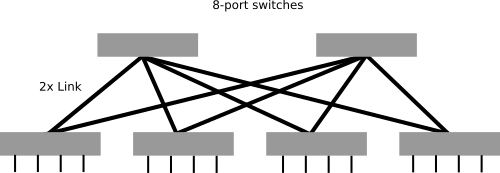
\includegraphics[width=0.85\linewidth]{Fat_tree_network.png}
  \caption{Two-tier Fat-Tree with 8-port switches ($k=8$; two \emph{switch} levels).
Lower tier (edge) switches attach $k/2=4$ hosts each and uplink $k/2=4$ ports to the upper tier (core).
Any host-to-host pair has multiple equal-cost up/down paths (up to $k/2=4$ via distinct core switches), enabling ECMP load balancing.
}
  \label{fig:Fat-Tree}
\end{figure}

ECMP provides path diversity in Clos/Fat-Tree fabrics by hashing flows to equal-cost paths; however, a single flow per neighbor exercises only one path. See (\ref{sec:implications-multipath}) for details and implications on ring design.


The goal of this research is to implement a dynamic approach for flow management in ring-based algorithms by adaptively increasing the number of flows used in communication whenever connection bandwidth is underutilized. 
By detecting when existing flows do not fully saturate the network capacity, the algorithm increases the number of parallel flows between two nodes in the ring, spreading traffic across more equal-cost paths to balance load and alleviate congestion.

In this work, we propose a bandwidth-aware multipath (multi-flow) ring semantics while adapting the number of per-neighbor flows to increase the bottleneck \emph{throughput} (achieved bandwidth) on a ring-based collective communication. We aim to establish three main contribution through this study:

\begin{itemize}[leftmargin=*]
%\item \textit{Model:} Per-edge parallelism with $k_e$ RDMA flows; define the per-edge \emph{achieved bandwidth} (application-layer throughput) $\bar{B}_e^{(k_e)}$ and the bottleneck $B_\star(\mathbf{k})$, yielding $T_{\text{ring}}(M,P,\mathbf{k})$.
\item A formal framework to analyze the performance of a ring-based collective communication with the aim of minimizing its completion time. 
\item The improvement of the bottleneck throughput connection on the ring by the establishment of parallel flows. These flows should be routed through disjoint paths by ECMP mechanism, thus, bypassing the congested links.
%\item \textit{Design:} RC-QP implementation using distinct 5-tuples to leverage ECMP, with flow-resizing only at coarse-grained control intervals.
\item A distributed local mechanism to adjust the transmission throughput of each node in the ring solely by sampling the incoming traffic throughput in the node. This distributed mechanism based on the local information of the nodes aims to maximize the total ring throughput and reduce the completion time of the collective operation.
%\item \textit{Controller:} A local per-edge rule that adjusts $k_e$ based on measured throughput on each ring edge, increasing $k_e$ when the edge appears persistently underutilized and decreasing $k_e$ when additional flows no longer improve throughput.
\end{itemize}


\section{Background}
\subsection{All-Reduce over Rings}
This section recalls the basic ring-based implementation of the \emph{All-Reduce} collective used for gradient synchronization in data-parallel training, and sets the notation used to analyze its cost.

\subsubsection{Model and Notation}
We consider $P\!\ge\!2$ processing units (ranks) indexed $\{p_0,p_1,\ldots,p_{P-1}\}$.
Each rank $p_i$ connects to its neighbors $p_{(i+1)\bmod P}$ and $p_{(i-1)\bmod P}$, forming a directed logical ring.
Each rank holds a buffer of size $M$ bytes that must be reduced across ranks and then replicated to all ranks.
Communication proceeds in fixed-size \emph{chunks} of $M/P$ bytes per step via neighbor-to-neighbor transfers only.
We use the standard $\alpha$–$\beta$ cost model: each step incurs startup latency $\alpha$ and transmission time proportional to size with factor $\beta$ (seconds per byte) \cite{thakur2005collectives}.
For later use, we write $\bar{B}_e$ for the steady-state \emph{application-layer throughput}
on logical-ring edge $e$ (bytes/s); a more precise definition is given in Section~\ref{sec:problem}.


\subsubsection{Ring All-Reduce (Reduce-Scatter + All-Gather)}
Figure~\ref{fig:ring-allreduce} illustrates the two-phase pipeline for $P=4$:
Fig. (a) shows a time-stepped three-worker Ring All-Reduce schedule adapted from ~\cite{yu2022scheduling}, and Fig. (b) shows the logical
partitioning and flow of chunks. The classic Ring All-Reduce algorithm has been widely discussed in the literature~\cite{thakur2005collectives,sergeev2018horovod,zong2025ibing}.


Ring All-Reduce consists of two pipeline phases:
\begin{enumerate}[leftmargin=*]
\item \textbf{Reduce-Scatter:} across $(P-1)$ steps, each rank sends one chunk to its clockwise neighbor and receives one from its counter-clockwise neighbor, accumulating a distinct chunk index per step.
\item \textbf{All-Gather:} in the following $(P-1)$ steps, the reduced chunks circulate so that all ranks reconstruct the full reduced buffer.
\end{enumerate}
During the Reduce-Scatter phase, each rank locally reduces the received chunk with its own data and forwards the updated partial result; during the All-Gather phase, no further reductions are performed and chunks are simply forwarded until every rank holds the complete reduced buffer, as in standard Ring All-Reduce descriptions~\cite{thakur2005collectives,sergeev2018horovod,zong2025ibing}.
Thus a ring of $P$ ranks performs $2(P-1)$ communication steps in total.
Each rank sends and receives $\tfrac{2(P-1)}{P}M$ bytes in total (approaching $2M$ for large $P$); for sufficiently large $M$ the pipeline sustains continuous link utilization on each link \cite{thakur2005collectives,sergeev2018horovod,zong2025ibing}.

\begin{figure}[t]
  \centering
  \subcaptionbox{Three-worker Ring All-Reduce schedule (RAR), showing reduce-scatter and all-gather phases (adapted from~\cite{yu2022scheduling}).\label{fig:ring-allreduce-rar}}%
  [0.48\linewidth]{%
    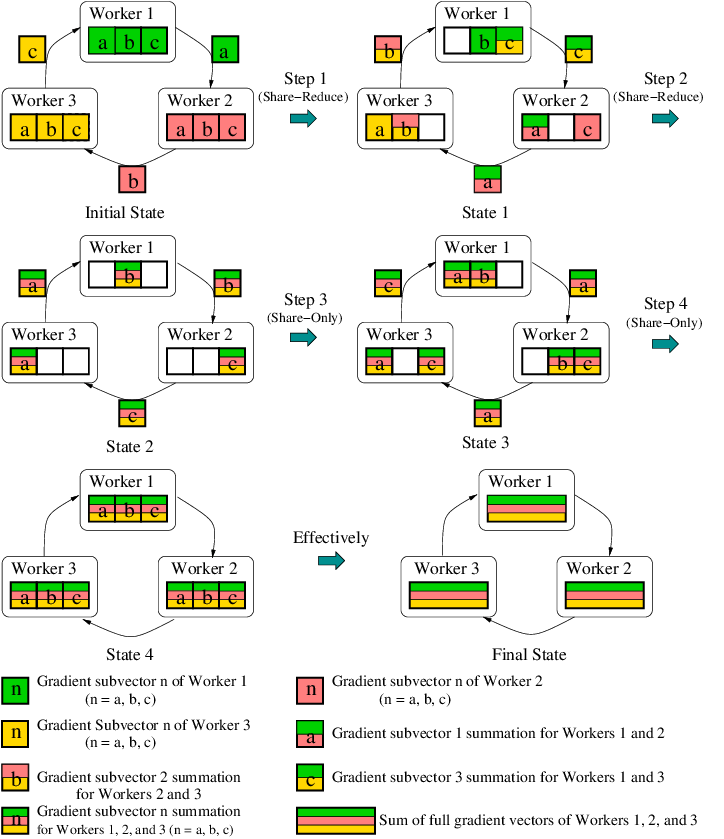
\includegraphics[width=\linewidth]{allreduce-RAR-process.png}}
  \hfill
  \subcaptionbox{Logical Ring All-Reduce for $P=4$.\label{fig:ring-allreduce-logical}}%
  [0.48\linewidth]{%
    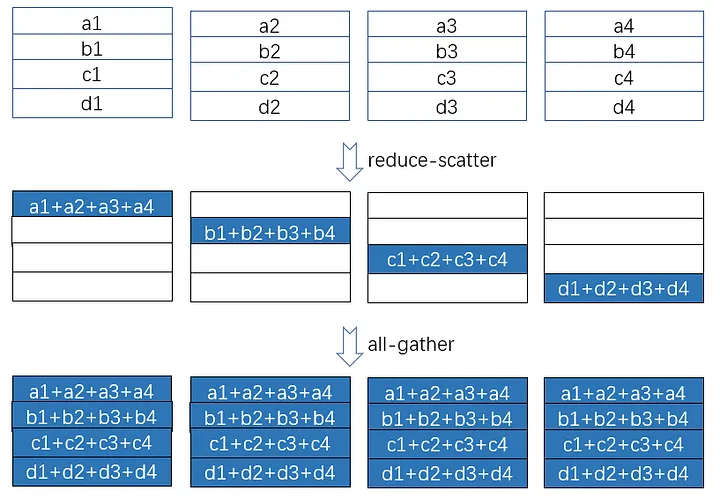
\includegraphics[width=\linewidth]{ring-allreduce.png}}
  \caption{Ring All-Reduce execution. Panel (a) shows a time-stepped three-worker schedule that makes the reduce-scatter and all-gather phases explicit, while panel (b) shows the logical partitioning and flow of chunks for $P=4$.}
  \label{fig:ring-allreduce}
\end{figure}



\subsubsection{Communication Cost and Completion Time (Bottleneck Model)}
Let $B_\star \triangleq \min_e \bar{B}_e$ be the per-step bottleneck across logical-ring edges.
Under the $\alpha$–$\beta$ model and full pipelining over chunks of size $M/P$ \cite{thakur2005collectives,sergeev2018horovod}, the completion time is
\begin{equation}
T_{\text{ring}}(M,P) \;=\; 2(P-1)\alpha \;+\; \frac{2(P-1)}{P}\cdot \frac{M}{B_\star}.
\label{eq:ring-time}
\end{equation}
For small $M$ the latency term $2(P-1)\alpha$ dominates; for large $M$ throughput dominates via $B_\star$.
A single slow edge (small $B_\star$) throttles the entire pipeline.
This expression follows the standard cost analysis of ring-based collectives in the MPI and deep learning literature \cite{thakur2005collectives,sergeev2018horovod,zong2025ibing}.
We later extend it to a per-neighbor multi-flow operation, yielding $T_{\text{ring}}(M,P,\mathbf{k})$ with bottleneck $B_\star(\mathbf{k})$ (Eq.~\ref{eq:ring-time-k}).



\subsubsection{Implications on Multipath Fabrics}
\label{sec:implications-multipath}
In Fat-Tree networks, ECMP maps each transport \emph{flow} (5-tuple) to a single path of equal-cost \cite{hopps2000rfc2992,leiserson1985fattree}.
A classic ring maintains one flow per neighbor, so only one path is used per hop; therefore $B_\star$ can be dictated by an unfavorable selection of congested paths.
To exploit path diversity while preserving the semantics of the ring, we allow each logical-ring edge $e$ to use $k_e$ parallel flows (distinct 5-tuples), yielding a bottleneck $B_\star(\mathbf{k})$.
For stability, $\{k_e\}$ are adjusted only at coarse-grained control intervals (e.g., between groups of collective iterations).


\section{Problem Formulation}
\label{sec:problem}
In a ring-based collective, every message chunk must traverse all neighbor-to-neighbor connections along the ring.
As a result, the overall throughput of the collective is bottlenecked by the slowest neighbor link.
Modern Clos/Fat-Tree data-center fabrics expose multiple equal-cost physical paths between any two ranks via ECMP, but a conventional ring typically uses a single transport flow per neighbor, so its throughput may be limited by congestion on a single unfavorable path.
To reason about using multiple flows per neighbor while preserving ring semantics, we formalize the underlying fabric and the induced logical neighbor links as follows.

We model the fabric as a directed multigraph $G=(V,E)$ where each link $e \in E$ is associated with a capacity $c_e$ (bytes/s).
For a pair of nodes $u,v\in V$, let $\mathsf{Paths}_{u,v}(G)$ be the set of all simple directed paths $P_{u,v}$ in $G$ between $u$ and $v$. Note that might be several paths in $\mathsf{Paths}_{u,v}(G)$ and at least one in case $G$ is connected. 
Assume  bandwidth $B(P_{u,v})$ as the maximum feasible bandwidth along path $P_{u,v} \in \mathsf{Paths}_{u,v}(G)$.
We define logical connection $L_{u,v}$ between a pair of nodes  $u,v\in V$ as a subset of $\mathsf{Paths}_{u,v}(G)$, i.e. $L_{u,v} \subseteq \mathsf{Paths}_{u,v}(G)$. 
A logical ring $R_(v_0,\dots,v_k)$ over nodes $(v_0,\dots,v_k)$ induces a set of logical connections between two cyclic consecutive nodes in $(v_0,\dots,v_k)$, i.e.  $\{L_{v_0,v_1},\dots,L_{v_k,v_0}\}$.



\begin{definition}[Achieved bandwidth of a logical connection]
Given a logical connection $L_{u,v}$ and the set of bandwidth $B(P_{u,v})$ (bytes/s) of $B(P_{u,v}$.
The achieved bandwidth on $L_{u,v}$ is the sum of the set of bandwidth $B(P_{u,v})$ 
\[
\bar{B}_{L_{u,v}} \;\triangleq\; \sum_{P_{u,v}\in L_{u,v} } B(P_{u,v}).
\]
\end{definition}


\begin{definition}[Ring bandwidth]
Given a logical ring $R_(v_0,\dots,v_k)$, its bandwidth is defined by the bottleneck bandwidth among its logical connections.
\[
\bar{B}_{R_(v_0,\dots,v_k)} \;\triangleq\; \min_{L_{u,v} \in R_(v_0,\dots,v_k)} \bar{B}_{L_{u,v}}.
\]
\end{definition}



\begin{definition}[Per-node input and output rates]
For each node $v$, $\bar{B}_{L_{u,v}}$and $\bar{B}_{L_{v,w}}$
denote its incoming and outgoing logical connection achieved bandwidth along the ring, respectively, and define
\[
\lambda_v^{\mathrm{in}} \;\triangleq\;
\bar{B}_{L_{u,v}},
\qquad
\lambda_v^{\mathrm{out}} \;\triangleq\;
\bar{B}_{L_{v,w}},
\]
as the corresponding input and output rates (bytes/s).
\end{definition}

These per-node rates will later serve as local measurements for the distributed controller that adjusts the logical connection size $|L_{u,v}|$ using only information observed at each node.
In particular, situations where $\lambda_v^{\mathrm{in}} > \lambda_v^{\mathrm{out}}$ indicate that the outgoing neighbor link of node $v$ is locally limiting the throughput, motivating an increase in the number of parallel flows on that link in our design.


%We choose integers $\{k_e\}_{e\in E_R}$ with $1 \le k_e \le k_{\max}$,where $k_{\max}\!\in\!\mathbb{N}$ is an implementation/resource cap per logical neighbor link (e.g., per-rank QP budgets or NIC limits).We write $\mathbf{k} \triangleq \{k_e\}_{e\in E_R}$ for the vector of flow counts on all logical neighbor links of the ring.


%Since every chunk in the ring must traverse all logical neighbor links, the steady-state throughput of the ring at a given configuration $\mathbf{k}$ is limited by its slowest logical neighbor link at that time.We therefore define the per-step bottleneck achieved bandwidth under flow vector $\mathbf{k}=\{k_e\}_{e\in E_R}$ as
%\[B_\star(\mathbf{k}) \;\triangleq\; \min_{e\in E_R} \bar{B}_e^{(k_e)}.\]


\paragraph{Completion time objective.}
For message size $M$ (bytes) and a logical ring $R_(v_0,\dots,v_P)$, the pipelined ring completion time is
\begin{equation}
T_{R_(v_0,\dots,v_P)}(M)
\;=\; 2(P-1)\alpha \;+\; \frac{2(P-1)}{P}\cdot\frac{M}{\bar{B}_{R_(v_0,\dots,v_k)}},
\label{eq:ring-time-k}
\end{equation}
where $\alpha$ is the per-step startup latency in the $\alpha$–$\beta$ model (seconds) according to \cite{thakur2005collectives,sergeev2018horovod}.

%\paragraph{Assumptions.}
%Throughout, we assume that ECMP spreads transport flows across equal-cost paths between ring neighbors and that standard RDMA congestion control (e.g., DCQCN/ECN) stabilizes the traffic.We also assume in-order delivery per QP and a chunk size chosen large enough (on the order of the bandwidth–delay product) so that the pipeline saturates for large messages $M$.

%\begin{problem}[Flow-count selection on a logical ring]
%Given a fabric $G=(V,E)$ with physical link capacities $\{c_f\}$, a logical ring $R$ over $P$ ranks with neighbor links $E_R$, a message size $M$, and an upper bound $k_{\max}$ on the number of flows per logical neighbor link, choose integers $k_e$ with $1 \le k_e \le k_{\max}$ for all $e\in E_R$ so as to maximize the bottleneck achieved bandwidth $B_\star(\mathbf{k})$. Equivalently, for fixed $M$ and $P$, this minimizes the ring completion time $T_{\text{ring}}(M,P,\mathbf{k})$ in Eq.~\eqref{eq:ring-time-k}.
%\end{problem}

In this proposal we aim to optimize the completion time $T_{R_(v_0,\dots,v_P)}(M)$ by designing an efficient distributed controller that adjusts the ring bandwidth ${\bar{B}_{R_(v_0,\dots,v_k)}}$ based only on the local rates $(\lambda_v^{\mathrm{in}},\lambda_v^{\mathrm{out}})$ of each node $v$.







\subsection{RDMA connection}
\label{sec:rdma}
%\subsubsection{Why RDMA in Practice}
In many HPC and distributed-training deployments, the logical ring edges are carried over Remote Direct Memory Access (RDMA) transports (InfiniBand or RoCEv2) to reduce CPU cycles via kernel-bypass and zero-copy and to increase achieved bandwidth; alternatives such as TCP/IP stacks are also used in practice. In this work we will implement the ring over RDMA for these efficiency reasons, while the cost decomposition in Eq.~\eqref{eq:ring-time} remains unchanged (the per-edge achieved bandwidth still determines the bottleneck $B_\star$) \cite{ibta2015vol1,nv-nccl-env}.

\subsubsection{RDMA Basics and Purpose}
RDMA enables a process to access a remote process’s registered memory directly via the NIC. We use Reliable Connection (RC) Queue Pairs (QPs), which provide reliable, in-order delivery \emph{per QP}. Each rank registers contiguous device buffers (obtaining LKey/RKey) and exchanges virtual addresses and RKeys with its two neighbors. Two communication types are relevant \cite{ibta2015vol1}:
\begin{itemize}[leftmargin=*]
  \item \textbf{Two-sided} \textit{SEND/RECV}: both endpoints post matching work requests; simple flow control, CPU involvement at both endpoints.
  \item \textbf{One-sided} \textit{WRITE/READ}: the initiator NIC directly writes to or reads from the peer’s registered memory; the remote CPU is off the data path. \textit{WRITE with immediate} additionally posts a lightweight signal to the receiver’s completion queue.
\end{itemize}

\subsubsection{Implementing the Ring with RDMA READ/WRITE}
Let ranks be indexed modulo $P$, with $\mathrm{next}(p)=(p+1)\bmod P$ and $\mathrm{prev}(p)=(p-1)\bmod P$. The message of size $M$ is partitioned into $P$ chunks of size $M/P$ and pipelined across steps.
\paragraph{WRITE–push (producer-driven).}
At step $s$, rank $p$ issues an \textit{RDMA\_WRITE} of chunk $j$ into a pre-allocated window at $\mathrm{next}(p)$ (optionally with immediate to signal arrival); the receiver reduces the arrived chunk into its local accumulator for index $j$.
\paragraph{READ–pull (consumer-driven).}
At step $s$, rank $p$ issues an \textit{RDMA\_READ} to fetch chunk $j$ from $\mathrm{prev}(p)$ and performs the local reduction; reads require no pre-posted receives; pacing is entirely local: the consumer keeps a small window $w$ of in-flight RDMA READs and issues a new READ only when a completion returns (i.e., a credit is freed).

RC guarantees in-order delivery within a QP. To avoid cross-QP reordering, each chunk is issued as a single work-request chain on one QP, with per-chunk sequence numbers checked on completion. 


\subsubsection{Multipath Implementation}
On RoCEv2 Clos/Fat-Tree fabrics, the RC QP number constitutes an input to the ECMP hash function causes ECMP to spread these different QP flows over multiple equal-cost physical paths \cite{hopps2000rfc2992,zhu2015dcqcn}.
In our setting, each logical ring edge between two neighboring ranks may use several parallel QPs (several flows). The total bandwidth of that edge is the bandwidth obtained by all its QPs together. Intuitively, using more QPs increases the chance that ECMP will route some of the flows through less congested physical paths, which can improve the effective throughput of that edge.

The ring algorithm itself remains simple: each data flow is pinned to a single QP, so RC ordering guarantees in-order delivery per flow.
Thus, our algorithm should divide the chunk into proper sub-chunks associated to a specific flow. Accordingly, the receiver should track only the flow order.ECMP runs transparently in the network and decides which physical path each QP uses; our algorithm only controls how many QPs are opened between neighbors and how they are used.



\section{Preliminary work}
\label{sec:motivation}
Modern training clusters often operate under oversubscription and transient failures. In such settings, the classic All-Reduce ring can suffer from cascading dependencies (“chain blocking”): congestion or a slow/failing hop throttles the entire pipeline. 
A recent work~\cite{wan2020rat} shows that All-Reduce completion time and throughput can be detrimentally impacted by contention and failure scenarios.

\begin{figure}[!t]
  \centering
  \subcaptionbox{Utilization vs.\ data size (adapted from IBING).\label{fig:ibing-data-size}}%
  [0.48\linewidth]{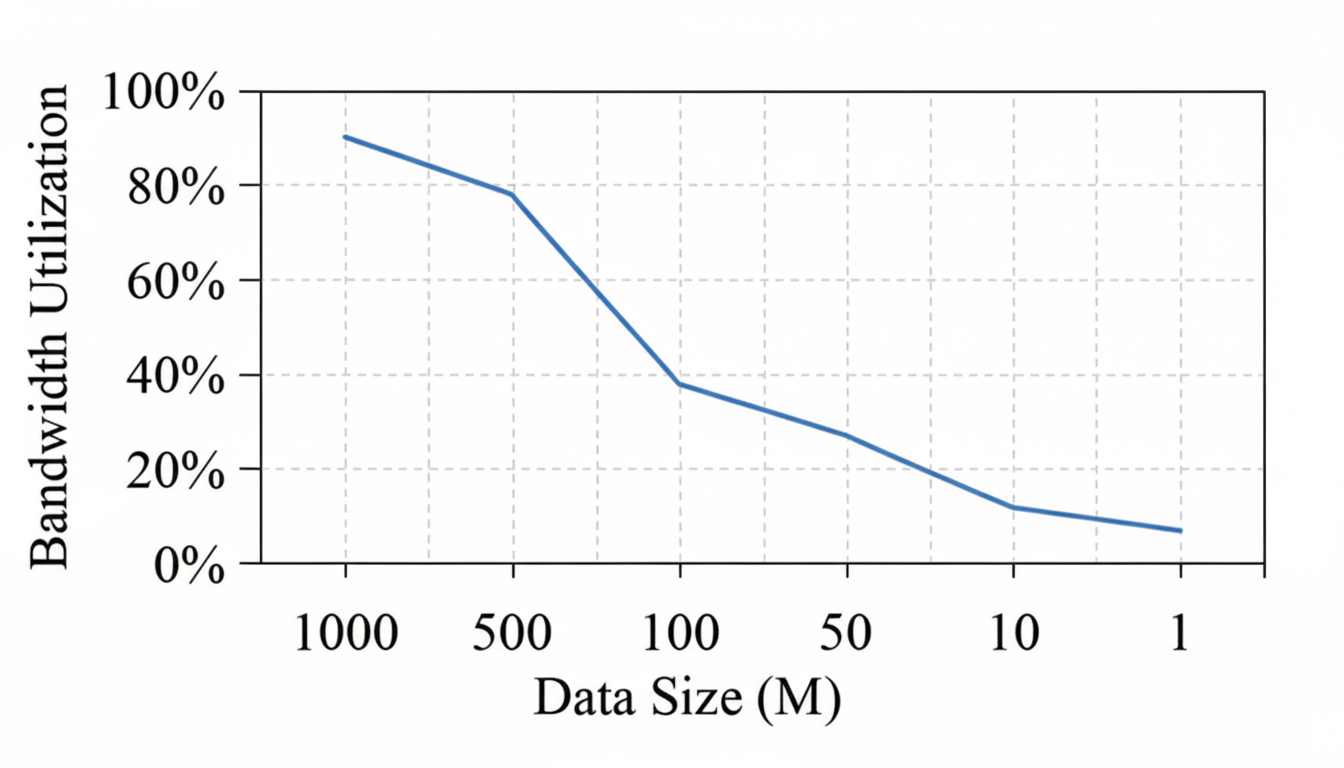
\includegraphics[width=\linewidth]{DATA-SIZE-RING.png}}
  \hfill
  \subcaptionbox{Utilization vs.\ number of nodes (adapted from IBING).\label{fig:ibing-nodes}}%
  [0.48\linewidth]{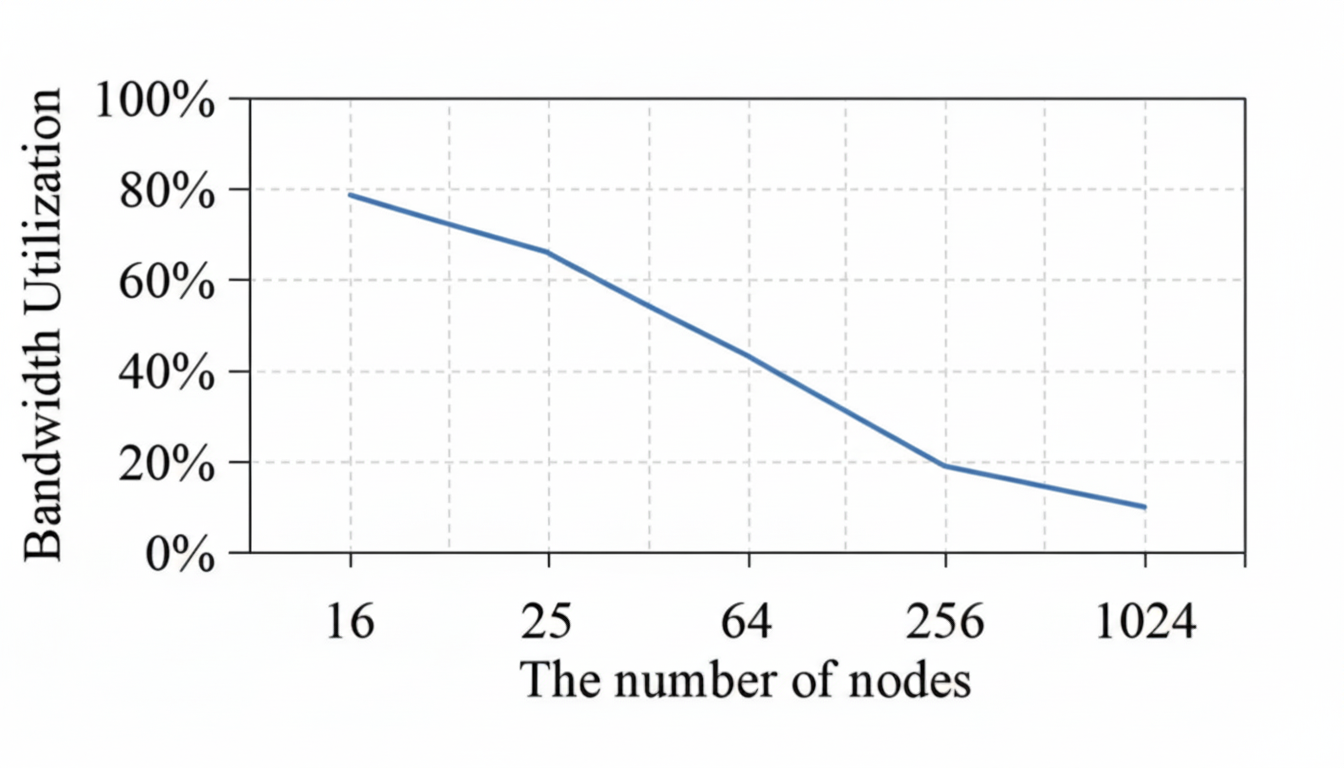
\includegraphics[width=\linewidth]{NODES-RING.png}}
  \caption{Single-flow ring underutilization in practice: degradation with smaller $M$ and larger $P$, aligning with the $B_\star$ bottleneck model.}
  \label{fig:ibing-evidence}
\end{figure}

A contributing root cause is how equal-cost multipath (ECMP) forwards traffic: a single transport flow is hashed onto one equal-cost path. Thus, the common single-flow-per-neighbor ring employs only one path per hop; unfavorable placements on congested links degrade the per-step bottleneck $B_\star$ that dictates completion time. Exploiting path diversity requires multiple parallel flows so that ECMP can distribute load across available paths \cite{hopps2000rfc2992,luo2020virtuoso}.

This observation motivates our design: preserve ring semantics but open $k$ parallel RDMA flows per neighbor and adapt $k$ online using a simple throughput-based rule evaluated over coarse-grained measurement windows.
By raising the per-edge achieved bandwidth $\bar{B}_e^{(k_e)}$ and, in turn, the bottleneck $B_\star(\mathbf{k})$, we aim to reduce $T_{\text{ring}}(M,P,\mathbf{k})$ on Clos/Fat-Tree fabrics with ECMP and ECN-based congestion control \cite{hopps2000rfc2992,zhu2015dcqcn}.

%\paragraph{Empirical evidence.}
Empirically (adapted from IBING \cite{zong2025ibing}), single-flow rings exhibit (i) utilization drop as message size decreases (latency/overheads dominate), and (ii) further degradation as the number of ranks $P$ grows (the bottleneck $B_\star$ dominates)—both consistent with Eq.~\ref{eq:ring-time} and motivating per-neighbor multi-flow (see Fig.~\ref{fig:ibing-evidence}).




%\noindent\textbf{Takeaway.}
Preserving ring semantics while opening $k$ per-neighbor RDMA flows (distinct 5-tuples) should improve $B_e^{(k_e)}$ and thus $B_\star(\mathbf{k})$, reducing $T_{\text{ring}}(M,P,\mathbf{k})$ on Clos/Fat-Tree fabrics \cite{zhu2015dcqcn}.





%----------------------------------------------------------
\section{Related Work}
Ring-based collectives are widely used in MPI and deep learning frameworks; classic analyses and optimizations appear in \cite{thakur2005collectives} and production practice in \cite{sergeev2018horovod,nv-nccl-env}. Under congestion and failures, ring All-Reduce can suffer from “chain blocking” and heavy-tailed completion times; alternative designs such as the Resilient Allreduce Tree (RAT) improve robustness and tail behavior under such conditions~\cite{wan2020rat}.

Beyond single-job collectives, Yu et al.~\cite{yu2022scheduling} study how to schedule multiple Ring All-Reduce learning jobs in multi-tenant GPU clusters, focusing on bandwidth allocation and job completion time rather than modifying the per-ring communication pattern itself.

On multipath fabrics, ECMP maps each flow (5-tuple) to one equal-cost path~\cite{hopps2000rfc2992}. RDMA deployments in Clos/Fat-Tree data centers typically rely on ECN-based congestion control for stability~\cite{zhu2015dcqcn}. At the transport layer, systems such as Virtuoso propose practical, scalable multi-path RDMA mechanisms that stripe traffic across several paths while remaining compatible with existing RDMA stacks \cite{luo2020virtuoso}. In contrast, our work operates at the collective-algorithm layer: we assume a standard RoCEv2+ECMP+ECN fabric and focus on how a ring All-Reduce can open and adapt the number of RDMA flows per logical ring edge. The goal is to raise the application-level bottleneck throughput $B_\star(\mathbf{k})$ of the ring, rather than redesign the underlying RDMA transport.


Topologically, Clos/Fat-Tree networks provide rich path diversity and scale-out with commodity switching \cite{leiserson1985fattree,alfares2008scalable}. Alternative high-scale designs (e.g., DCell, BCube, Dragonfly) illustrate other path-diverse fabrics \cite{guo2008dcell,guo2009bcube,kim2008dragonfly}; we focus on Clos/Fat-Tree with ECN/DCQCN, where ring semantics and ECMP interplay directly.

A related strand of work optimizes ring-based collectives by modifying the logical topology, for example by constructing multiple edge-disjoint or ingress-balanced rings to alleviate congestion hot spots in Clos/Fat-Tree fabrics \cite{zong2025ibing}. Other schemes replace rings altogether with more resilient tree-based structures such as RAT \cite{wan2020rat}. These approaches change the collective topology, whereas we keep a single logical ring and instead multiplex several RDMA flows per logical edge to exploit ECMP path diversity.

A complementary line of work, known as \emph{collective synthesis}, designs collective algorithms automatically. Given a network topology and a target operation such as All-Reduce, systems like SCCL and TACOS~\cite{cai2021sccl,won2024tacos} search for communication schedules that nearly saturate the available bandwidth. Our work is orthogonal: we keep the ring algorithm fixed and instead exploit path diversity on each logical ring edge via adaptive multi-flow RDMA, so that a multi-path ring can serve as a building block within synthesized schedules.



%----------------------------------------------------------
\section{Research Plan}
%----------------------------------------------------------

The proposed research will be carried out in four stages, combining an instrumented single-flow baseline, a multi-flow ring with a local controller, and an experimental evaluation on Clos/Fat-Tree fabrics:

\begin{enumerate}[leftmargin=*]
  \item \textbf{Stage 1 – Single-flow baseline.}
        Implement a single-flow ring All-Reduce over RDMA
        (Section~\ref{sec:rdma}) and instrument it to measure
        per-edge throughput $\bar{B}_e$, bottleneck throughput $B_\star$, and
        completion time $T_{\text{ring}}(M,P)$ for different message sizes $M$
        and numbers of ranks $P$. Use these measurements to validate and
        calibrate the model and to select practical defaults for chunk size
        and the number of in-flight operations.

  \item \textbf{Stage 2 – Multi-flow ring and local controller.}
        Extend the baseline to support $k_e \ge 1$ parallel RDMA flows per
        logical ring edge $e \in E_R$, using distinct 5-tuples (RC QPs) so that
        ECMP can exploit multiple physical paths. Define a simple chunk-to-QP
        assignment that preserves per-chunk ordering, and implement a local
        throughput-based controller at each rank that periodically estimates
        $(\lambda_p^{\mathrm{in}},\lambda_p^{\mathrm{out}})$ and adjusts $k_e$
        only at coarse-grained control intervals.

  \item \textbf{Stage 3 – Experimental evaluation on multipath fabrics.}
        Evaluate the single-flow and multi-flow rings on a Clos/Fat-Tree fabric
        with ECMP and ECN-based congestion control. Measure
        $\bar{B}_e^{(k_e)}$, $B_\star(\mathbf{k})$, and
        $T_{\text{ring}}(M,P,\mathbf{k})$ for different $(M,P,\mathbf{k})$
        both without cross-traffic and under controlled background load.
        Compare median and tail completion times, bandwidth utilization, and
        the overhead of maintaining multiple flows (QPs, CPU/NIC usage).

  \item \textbf{Stage 4 – Analysis, guidelines, and extensions.}
        Analyze the experimental results and derive design guidelines:
        for which ranges of $(M,P)$ and network conditions a multi-flow ring is
        beneficial, and how many flows per neighbor are typically sufficient.
        If time permits, extend the approach to other bandwidth-bound
        collectives (e.g., AllGather) and evaluate robustness under transient
        link slowdowns or failures that emulate realistic data-center behavior.
\end{enumerate}



\newpage
%----------------------------------------------------------
\section*{Acknowledgments}
%----------------------------------------------------------
\printbibliography
\end{document}